\section{Head Mounted Display}
\label{sec:hmd}

\begin{figure}[]
\centering
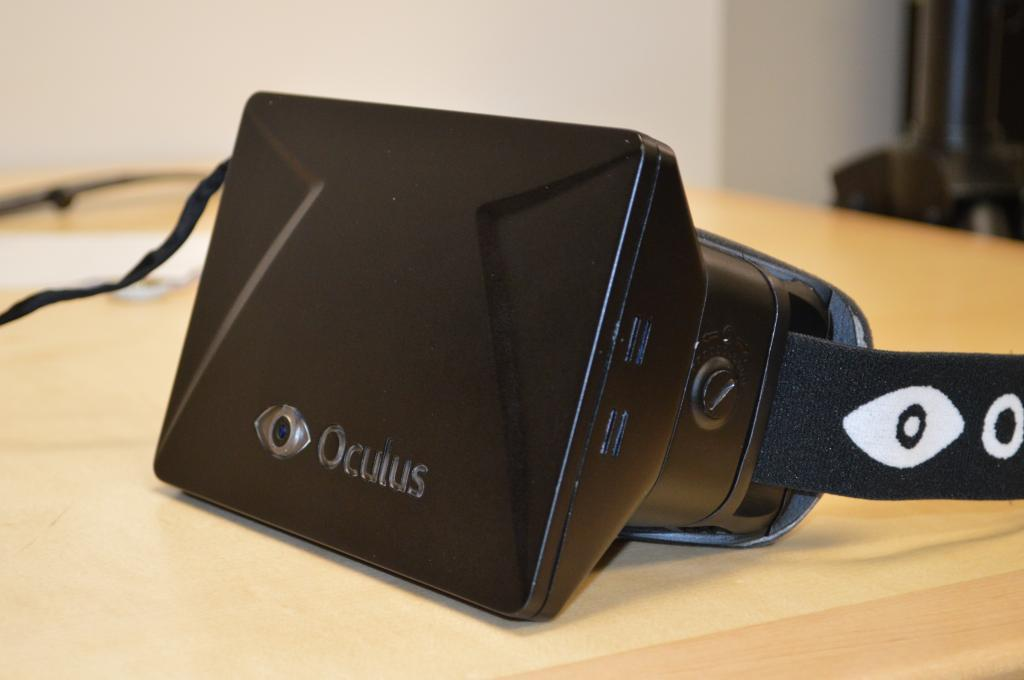
\includegraphics[width=0.5\textwidth]{oculus.jpg}
\caption{Oculus Rift Development Kit 1. 
\cite{website:pcworld}}
\label{fig:oculus}
\end{figure}

\begin{figure}[]
\centering
\includegraphics[width=0.5\textwidth]{stereo_lens.png}
\caption{Above is a stereoscopic split screen view also rendered with barrel distortion.
    Below, are the magnifying lenses of the oculus headset.
Frames displayed on the Oculus screen appear normal when the headset is worn.}
\label{fig:stereo}
\end{figure}


The Oculus Rift seen in Fig. \ref{fig:oculus} is the current state of the art
in HMD VR technology. There are several elements to the device that allow the
Oculus to provide the most immersive visual VR experience thus seen.

The first is speed.  The VR realism is directly tied to this response time, and
the Oculus overcomes the problem of graphical latency, which has plagued all of
its predecessors. It does so by sampling data from its 3-axis gyro,
accelerometers, and magnetometers at a rate of 250Hz \cite{website:roadtovr};
the newer version is said to have a sampling rate of 1000Hz. Its ability to
gather data so quickly from its propriocetive sensors allows the graphics on
the display to be adjusted to correspond to real time head movements. Secondly,
the Oculus renders scenes split screen stereoscopic 3D. The left eye sees the
left half of the screen and the right eye sees the right half, which is
consistent with human perception. Leveraging split screen stereo greatly
enhances the perceived 3D effect. Finally, the Oculus uses large magnifying
lenses in order to completely encompass the user's peripheral vision and
greatly expand the user's field of view. All of these aspects must be
considered when developing the graphics of the scene. Fortunately the C++ SDK
provides sufficient overhead to deal with them, allowing graphics developers to
stay focused on developing graphics instead of worrying about the details of
implementation.

The most simple applications one can develop for the Oculus are created using
basic OpenGL \cite{website:opengl}. The only caveat is that a separate
framebuffer must be bound to the context for off-screen rendering, and each
scene must be rendered twice, once for each eye. The framebuffer must have a
texture bound to it as well, which is written to at the last stage of the
conventional pipeline.  The Oculus SDK provides parameters for constructing the
texture, which can be accessed programmatically. The Oculus SDK will then take
the data placed in the texture and perform the post-processing for distortion
processing after the GLSL shaders, if any, have been executed.

Human eye pupils are approximately 65 mm apart.  This interpupillary distance
(IPD) must be taken into consideration for configuring the in-application
camera. Therefore, each scene is rendered twice, once for the virtual camera on
the left, and once for the virtual camera on the right. Both of which are
subject to a translation with respect to one another causing the stereoscopic
effect. The programmer must apply this translation to the view in each frame.
The translation is provided by the SDK.

The use of the large magnifying lenses causes the image succumbs to a great
deal of pincushion distortion. To rectify this distortion, the software must
apply an equal and opposite amount of barrel distortion. The final image
rendered to the Oculus's display can be seen in Fig. \ref{fig:stereo}. For the
remainder of this paper, when discussing the camera view, this refers to the
single camera model provided to the Oculus SDK before the post processing
occurs. 

As advanced as the Oculus is, it is not without limitations.  While it is able
to track rotation effectively, it provides no means of tracking translation.
Those familiar with the company should find themselves critical, as they know
that the newer version of the Oculus does provide position tracking as well.
Be that as it may, its position tracking is limited as it is designed to track
within a small volumes, for instance, the space just in front of a desk. In
addition, it provides not ability track any other objects other than itself.

Graphics is known as the inverse problem to computer vision. Where computer
vision seeks to extract information about an environment from an image,
graphics seeks to extract information from an environment to construct an
image. What gives computer graphics the illusion of position and depth is a
mathematical process of constructing a series of transformations taking
arbitrary points from one frame of reference to another.  A perspective
projection transform is applied at the end of the sequence once all the objects
are defined with respect to the viewer, in order to create the final image.

The location of all the particles in an object can be defined with respect to
some frame of reference usually referred to as the model. If one observes the
object from some alternative location and orientation with respect to the model
frame, one can construct a transformation to take points from the model frame
to the view frame.

\[
\begin{pmatrix} x \\ y \\ z \\ 1 \end{pmatrix}^{view} = 
    \begin{pmatrix}
        r_{1} & r_{2} & r_{3} & t_{x} \\
        r_{4} & r_{5} & r_{6} & t_{y} \\
        r_{7} & r_{8} & r_{9} & t_{z} \\
        0 & 0 & 0 & 1
    \end{pmatrix}^{view}_{model}
    \times
\begin{pmatrix} x \\ y \\ z \\ 1 \end{pmatrix}^{model}
\]



Manipulating the pose of this view frame will be discussed in Section
\ref{sec:mocap}. Normally, the orientation of the Oculus is constructed from
the measurements provided by its sensors, and is used directly as the
orientation of the view frame.

\begin{figure}[]
\centering
\includegraphics[width=0.5\textwidth]{view_model.png}
\caption{Two frames of reference, the view and the model. The orientation and
position of the view frame corresponds to the camera view. The axis are
defined in the graphics convention. Red is \emph{x}, green is \emph{y}, 
and blue is \emph{z}.}
\label{fig:worldview}
\end{figure}

